%%%%%%%%%%%%%%%%%%%%%%%%%%%%%%%%%%%%%%%%%%%%%%%%%%%%%%%%%%%%%%%%%%%%%%%%%%%%%%%%%%%%%%%%%%%%%%%%%%%
\chapter{Background} \label{ch:Concepts}

\section{Introduction}
In this chapter we will discuss some important concepts relevant to this dissertation. This include an overview of both \ac{LiDAR} and \ac{FMCW} radar technologies, the components needed to achieve autonomous navigation,  and a quick overview of the \ac{ROS} platform.

\section{\ac{LiDAR} vs \ac{RADAR}}

In order to do complex tasks and compute different complex algorithms robots require some type of information that relates to its state and environment. This information comes from its sensor sources.
The most typical type of sensors used for perception are usually laser range finders (\ac{LiDAR}), sonar and the a rgb-d camera. However the new emerging \ac{mmWave} \ac{FMCW} radar technology with high frequency and bandwidth 77-81 GHz is now beginning to be suitable for use in robotic applications. In the following  sections we will give a brief overview of current work being done using \ac{LiDAR} and \ac{FMCW} \ac{RADAR}, how they work, and what advantages and disadvantages each sensor has.

\subsection{LiDAR}
\ac{LiDAR} has been a staple in sensing technology in recent history. It has almost an  unlimited  number of applications \cite{lidar100uses} due to its generation of dense data. Some of the most standing out ones are in autonomous vehicles and robotics. 
\subsubsection*{Autonomous Vehicles}

The use of \ac{LiDAR} in autonomous vehicles has been a common trend for a while now (Fig. \ref{fig:lidarcar}). The insanely accurate depth information combined with a high field of view provided by \ac{LiDAR} enables the development of advanced navigation systems that are able to perform self-driving.
 
 
\begin{figure}[h] 
\centerline{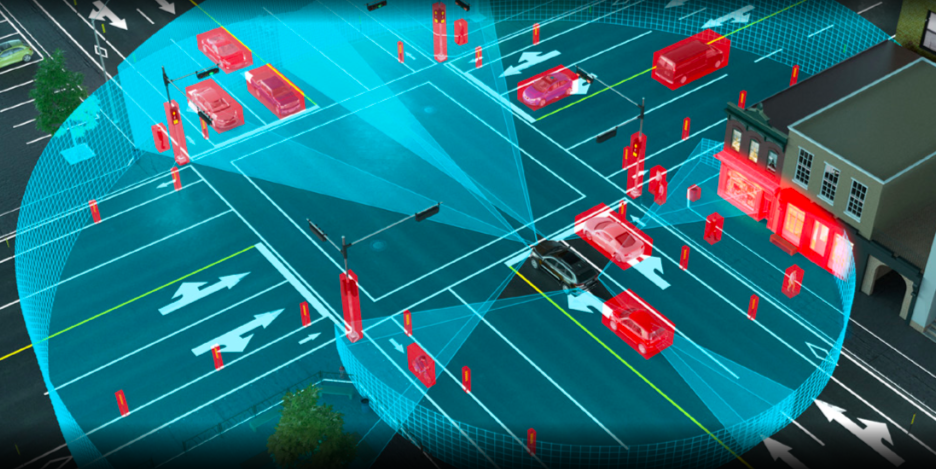
\includegraphics [width=0.7 \textwidth]{imgs/chapter2/lidarcar.png}}
\caption{Example of \ac{LiDAR} technology being used for road perception \cite{lidarcar}}
\label{fig:lidarcar}
\end{figure}

Some application examples of this include \cite{lidarperception}  where it was implemented a perception system for ground vehicles based on \ac{LiDAR} using segmentation, clustering and tracking techniques.  However, it was noted that it was hard to distinguish between closely  separated obstacles adding that a movement detection algorithm should be implemented to solve this problem. 

In \cite{car2dlidar} a low cost solution for object detection, classification and ranging is  proposed by the use of an inexpensive 2D pulsed light \ac{LiDAR}. The system was able to provide reliable detection of 1 meter wide obstacles at distances less than 10 meters.


However there are some concerns about this type of technology. CEO of Tesla, Elon Musk has been very critical of it. Recently, at Tesla’s first Autonomy Day event  he said \textit{"Anyone relying on \ac{LiDAR} is doomed. Doomed!"} \cite{elon}. He believes that cameras, radar and ultrasonic sensors are the future for car visions systems. 
\subsubsection*{Robotics}
\ac{LiDAR} is also one of the major sensory component for robotics (Fig. \ref{fig:robotslidar}). Various robots rely on it for autonomy and navigation.
\begin{figure}[h] 
    \begin{minipage}[b]{.49\linewidth}
        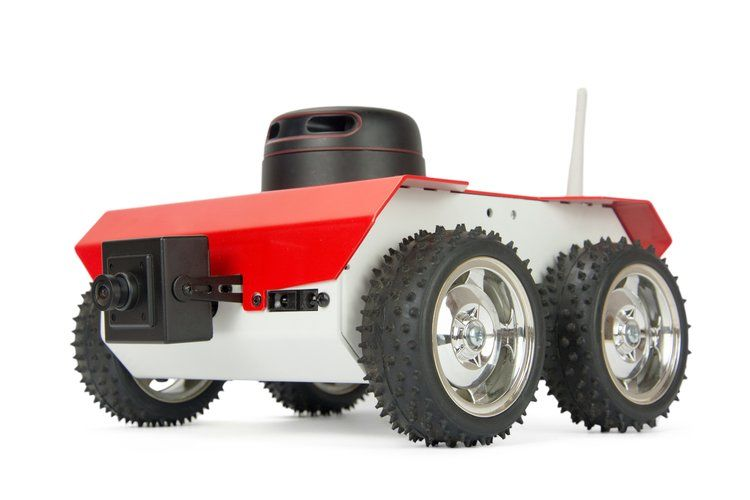
\includegraphics[height=5cm,width=\linewidth]{imgs/chapter2/robot1.jpg}
        \subcaption{ROSbot - Autonomous Robot with Laser scanner RPLiDAR A2 \cite{robot1}}
    \end{minipage}
    \begin{minipage}[b]{.49\linewidth}
        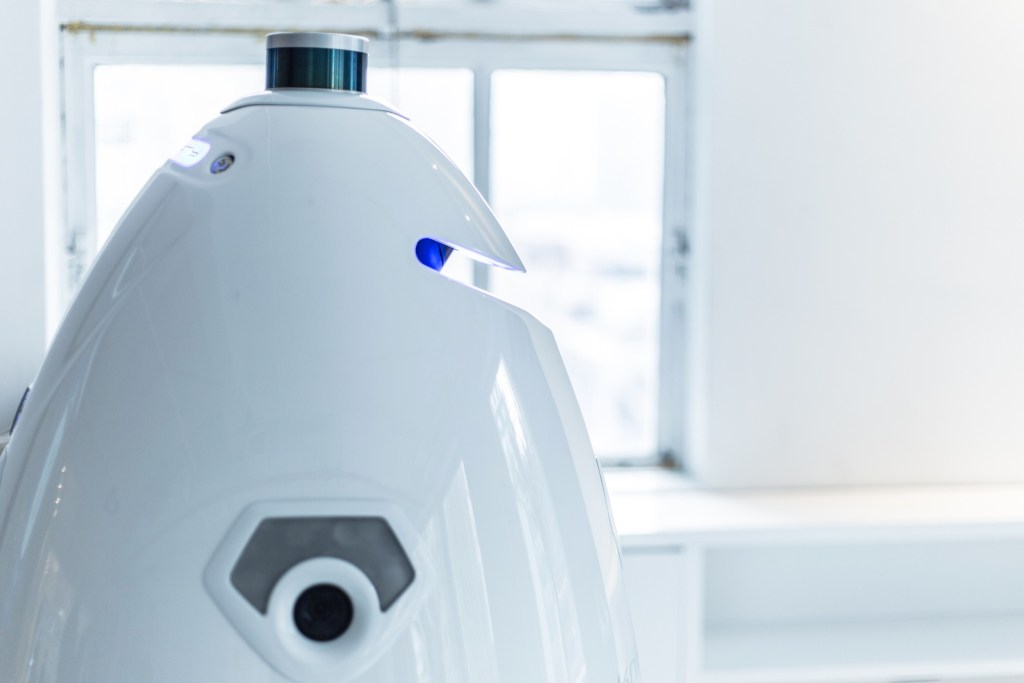
\includegraphics[height=5cm,width=\linewidth]{imgs/chapter2/robot2.jpg}
        \subcaption{Knightscope autonomous security robot with a Velodyne \ac{LiDAR} Puck \cite{robot2}}
    \end{minipage}
    \caption{Different robots using \ac{LiDAR}}
    \label{fig:robotslidar}
\end{figure}
\cite{marder2010office}  the PR2 robot was able navigate autonomously for 26.2 miles in an office like environment. During the task, the robot was able to avoid  shelves, tables, chairs and people as well as go
through narrow spaces. The sensor source used in this case was the Hokuyo UTM-30LX Scanning Laser Rangefinder and the navigation system developed is now known as the \ac{ROS} navigation stack. However it was noted that the robot had difficulty detecting low long obstacles.
In \cite{lidar2019ros} an autonomous robot mobile robot is constructed  using a 2D \ac{LiDAR} sensor. 

%%ADD ROBOT INDOOR NAVIGATION
\subsubsection{Operating Principle}
The way \ac{LiDAR} technology works is very straightforward, just emit a laser beam and wait for it to bounce back. Based on the proprieties of the reflected signal we can determine the range of the obstacle it hit. By spinning the mirrors at different angles (scanning) we get a set of points cloud that give angle and depth information about the environment. There are two main different operating principles to do this, \textbf{Time of Flight} and \textbf{Phase Based}.
\subsubsection*{Time of Flight}
 In this approach a pulse of light is transmitted, when this is done an internal clock is started. The pulse is captured by a photodetector which triggers the clock to stop. Being $\tau$ the time it took for the reflected signal to  comeback and assuming it traveled at approximately the speed of light ($c$) then the distance of the object $d$ is equal to:
\begin{equation}
    d=\frac{\tau c}{2}
\end{equation}
This method produces very accurate results for a wide range but requires high precision clocks. However greater  range capability leads to slower update rates since it has to wait more time for the pulse to comeback.
It is typically not used for robotics since this types of systems have very high cost.
\subsubsection*{Phase Based}
A more affordable approach  is based on modulating the intensity of the laser at a specific frequency. Figure \ref{fig:cwlidar1} showcases the resulting sinusoidal wave that is sent and the respective returned signal. 
\begin{figure}[h] 
\centerline{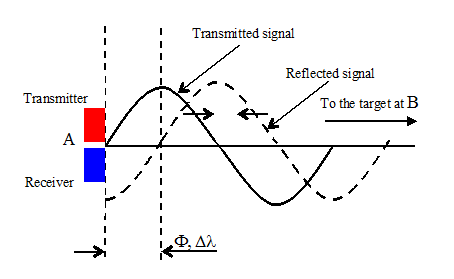
\includegraphics [width=0.7 \textwidth]{imgs/chapter2/cwlidar1.png}}
\caption{Phase comparison method of measuring distance \cite{cwlidar}}
\label{fig:cwlidar1}
\end{figure}

Being $\Phi$ the phase difference between the two and $\lambda_m$ the wavelength of the sinusoid then the distance of the object is given by:
\begin{equation}
    d=\frac{\Phi \lambda_m}{4 \pi}
\end{equation}
This means that the maximum unambiguous distance that can be measured is  $\frac{\lambda_m}{2}$, and its range resolution depends upon the resolution of the phase difference measurement as well as the wavelength used. Almost all robots use this type of \ac{LiDAR} since it is usually cheaper and as a faster update rate.
%difficult to generate continuous wave of high energy

\subsubsection{Limitations}
\ac{LiDAR} technology has some problems associated with it, they are:
\begin{itemize}
\item{They are usually expensive sensors costing thousands or even tens of thousands of dollars a piece}  
\item{Range and perception}  
\item{bulky}  
\item{robustness} 
\item{Particular difficult cases} 
\end{itemize}

\subsection{FMCW Radar}

\subsubsection{History and applications}
\subsubsection{Applications}
\subsubsection{advantages vs disadvantages}
lack the angular resolution 


%GIVE OVERVIEW OF THE CURRENT SENSORS LEADING INDOOR NAVIGATION.

\section {Navigation Concepts}
There are four main problems associated with robotic autonomous navigation. They are Cognitive Mapping, Localization, Path Planning and Motion Control \cite{baranov2014}.  various algorithms have been developed over the years to combat this problems. In the sections bellow we give a brief overview of the more popular solutions.

\subsection{Mapping}

Creating a map in ROS is typically done by using an improved version of  Rao-Blackwellized particle filters such as the ones described in \cite{grisetti2007improved}. This approach has proven to be an effective way to solve the \ac{SLAM} problem and will be used later on in this work to produce a valid map of our indoor environment.
%gmapping, slam, eurico LASER
\subsection{Localization}
With the grid map built we now need to estimate the robot's position in said map. 
An easy solution to this problem is relying on the robot's odometry information inferred by the robot's encoders and inertial sensors such as accelerometers and gyroscopes. This kind of dead reckoning is an easy and low cost solution for the localization problem. However since the sensor data is integrated over time, this leads to the accumulation of errors which make this approach not feasible for long navigation tasks. 
To fix this issue various algorithms were developed being the most popular ones based on particle filters.
The \ac{AMCL} algorithm  is the standard choice in this case. It takes into account a group of particles, each one corresponding to a certain robot state (position and orientation in this case). As the robot moves the least probable states are filtered out and  the particles should over time converge on the actual position of the robot.  
\subsection{Path Planning}
Assuming the robot can localize itself on the map with a reasonable error we can start sending navigation goals to the robot. To reach the goal the robot must be able to find a path that optimizes the travel distance while avoiding obstacles. The outputted plan can vary depending on the algorithm used. In our case we will use the well known dijaktra algorithm.
\subsection{Motion Control}
After the optimal plan is computed the final step is to determine the best velocity command that will be sent to the base.  The ROS navigation system follows a similar approach to the one used in \cite{gerkey2008planning}. A set of velocities are simulated during a given set of time and the corresponding predicted trajectories are  computed. For each trajectory it is calculated a determined cost given by a cost function  taking into account 
\section {\ac{FMCW} radars working principle}
In order to retrieve the best data for our application we first need to understand how the radar works. The following sections will try explain how the radar calculates the range, velocity and angle of an object.
\subsection{range Detection}
An \ac{FMCW} radar transmits a signal called a “chirp”. A chirp is a sinusoid whose frequency  increases linearly with time.
%% put A t and f t plot
A chirp is characterized by a start frequency (fc), bandwidth (B) and duration (Tc). The slope (S) of the chirp is the rate at which the frequency of the chirp increases and is given by:
\begin{equation}
    S=\frac{B}{T_c}
\end{equation}
%%PUT SOME TEXT
Object detection follows this steps:
\begin{enumerate}
    \item The chirp is transmitted by the TX antenna
    \item The chirp is reflected off an object and the reflected chirp is received at the RX antenna
    \item The RX signal and TX signal are ‘mixed’ and the resulting signal is called an ‘IF signal’
\end{enumerate}


%%PUT IMAGE
%%%When the transmitted chirp encounters an object it will reflect back to the radar and will be captured by the RX antenna.
The RX signal is a sum of delayed versions of the TX signal. This means that the resulting \ac{IF} signal will be a combination of sinusoids. Each of this correspond to a reflection of an object. For object $i$ the corresponding frequency $f_i$ is equal to:
\begin{equation}
    f_i=S\tau_i
\end{equation}
Where $\tau_i$ is equal to the round trip delay of the wave and is equal to:
\begin{equation}
    \tau_i=\frac{2d_i}{c}
\end{equation}
Where $d_i$ corresponds to the distance of the object to the radar and $c$ the speed of light.
%% PUT image
Putting this together the distance to the object $i$ is given by:
\begin{equation}
    d_i=\frac{f_ic}{2S}
\end{equation}

 So to determine the range of all objects detected we only need to find the according frequency components in the \ac{IF} signal. To do this the analog signal is first sent to an \ac{ADC} and with the resulting digital output the \ac{FFT} is computed by a \ac{DSP}. Each peak in the \ac{FFT} that meets a certain \ac{SNR} threshold corresponds to a different range detection. 
 
 However since the \ac{ADC} has a limited sampling rate, the valid range of frequencies in the \ac{FFT} is also limited, this means there is a maximum amount of range the radar can detect.
The range resolution is also finite since the \ac{FFT} has a limited amount of samples. In short, the higher the bandwidth of the chirp the better resolution we get.
 
\subsection{velocity Detection}
This type of radar also provides an estimate on the radial velocity for each detected range. To do this we need more than one chirp. A set of N chirps is called a frame. The radar constantly sends this frames, each one corresponding to an observation. Since the time between frames is so low the corresponding range-\ac{FFT}s will have  identically located peaks (the same obstacle is in the same range for all chirps in a frame) . However this set of peaks have different phases between each other. By calculating a second \ac{FFT} (Doppler-FFT) of this vector of phases we can extrapolate a set of velocities  for each range detection. In the end we get a matrix that relates radial velocity and range.
\subsection{angle Detection}
For this type of de
 %A cluster is just a subset of points of the cloud that are close together. This takes into account if a point has alot of close neighbours. If it has than it is considered a cluster.  
- New Technology
- New possibilities
\section {ROS}
Creating software for robotic applications is not an easy task to do from scratch. It usually involves very complex code to achieve even the simplest applications due to the wide variety of hardware and data that robots rely on. \ac{ROS} fixes this issue by being an open-source general purpose framework for robotics. It provides hardware abstraction, device drivers, tools for introspection, message-passing and more. This greatly facilitates the entrance of new developers to learn and do research in this field.
\subsection{ROS architecture}
The \ac{ROS}  architecture is based on a peer to peer network between processes usually referred to as \textit{Computation Graph}.
This structure is composed by:
\begin{itemize}
\item \textbf{Nodes} - Processes that perform computation.
\item \textbf{Messages} - ROS predefined data type used to communicate between nodes. 
\item \textbf{Topics} - Nodes can send messages by publishing to a topic or receive them by subscribing to a topic. 
\item \textbf{Master} - Provides registration of names (helps nodes find each other).
% V
\item \textbf{rosout} - ROS equivalent of stdout 
\item \textbf{roscore} - Master+rosout+parameter server. 
%X
\end{itemize}

%%REVER ISTO

Figure \ref{fig:rosgraph} gives a brief overview of how each of this concepts are put together and  generate the in ROS  computation system.

\begin{figure}[h] 
\centerline{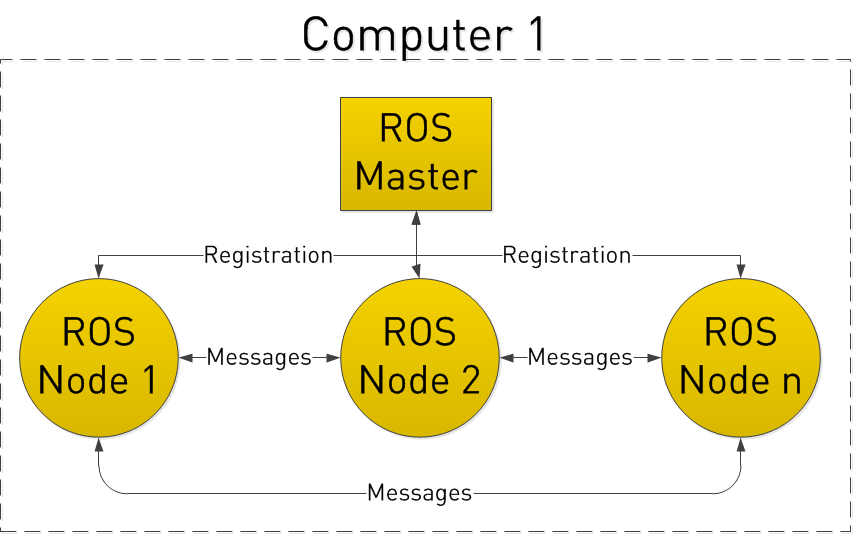
\includegraphics [width=0.5 \textwidth]{imgs/chapter2/rosgraph.png}}
\caption{ROS communication architecture overview \cite{rosbasics}}
\label{fig:rosgraph}
\end{figure}


